% \documentclass[journal]{IEEEtran}
\documentclass[12pt,journal,draftclsnofoot,onecolumn]{IEEEtran}
\IEEEoverridecommandlockouts

% remove colon after subsubsection, use spacing instead
\makeatletter
\renewcommand{\@IEEEsectpunct}{\quad}
\makeatother

\makeatletter
% add a small spacing *before* subsections
\let\origsubsubsection\subsubsection
\renewcommand\subsubsection{\@ifstar{\starsubsubsection}{\nostarsubsubsection}}

\newcommand\nostarsubsubsection[1]
{\subsubsectionprelude\origsubsubsection{#1}}

\newcommand\subsubsectionprelude{%
  \vspace{6pt}
}
\makeatother

% change default font to charter
% \usepackage{charter}
% \usepackage[bitstream-charter]{mathdesign}
% \usepackage{XCharter}
\usepackage{amsfonts}

% Fixing IEEEtran.cls bug with [english]{babel}
\makeatletter
\def\markboth#1#2{\def\leftmark{\@IEEEcompsoconly{\sffamily}\MakeUppercase{\protect#1}}%
\def\rightmark{\@IEEEcompsoconly{\sffamily}\MakeUppercase{\protect#2}}}
\makeatother

% \usepackage{t1enc}

\usepackage{listings}
\usepackage{multirow}
%\usepackage[utf8x]{inputenc}
\usepackage[english]{babel}
\selectlanguage{english}
\usepackage{color}
%\usepackage{caption}
\usepackage{cite}
\usepackage[pdftex]{graphicx}

% \usepackage{subfig}
\usepackage{subcaption}
\usepackage{amsmath}

\usepackage{mathtools}
\DeclarePairedDelimiter\ceil{\lceil}{\rceil}
\DeclarePairedDelimiter\floor{\lfloor}{\rfloor}

\usepackage{amsfonts}
\usepackage{array}
\usepackage{verbatim}
\usepackage{listings}
\usepackage[hidelinks]{hyperref}
\usepackage{url}
\usepackage{enumerate}
\usepackage{multirow}

\usepackage{siunitx}
\usepackage{epsfig}
\usepackage{epstopdf}
\usepackage{multicol}% http://ctan.org/pkg/multicols
\usepackage[font=footnotesize]{caption}
% \usepackage[font=scriptsize]{subcaption}
% Tikz
\usepackage{tikz}
\usepackage{pgfplots}
\pgfplotsset{compat=newest}
\pgfplotsset{plot coordinates/math parser=false}
\newlength\fheight
\newlength\fwidth
\usetikzlibrary{patterns,decorations.pathreplacing,backgrounds,calc}
\definecolor{SchoolColor}{RGB}{0.71, 0, 0.106}%181,0,27} unipd red
\definecolor{chaptergrey}{rgb}{0.61, 0, 0.09} % dialed back a little
\definecolor{midgrey}{rgb}{0.4, 0.4, 0.4}
\definecolor{chaptergreen}{rgb}{0.09, 0.612, 0}
\definecolor{chapterpurple}{rgb}{0.522, 0, 0.612}
\definecolor{chapterlightgreen}{rgb}{0, 0.612, 0.522}

%\raggedbottom

% Pseudocode
\usepackage[ruled, vlined]{algorithm2e}

\SetKwRepeat{Do}{do}{while}
\SetKwBlock{wpPa}{with probability $P_A$}{end}
\DontPrintSemicolon
% \usepackage{algorithm}
% \usepackage[noend]{algpseudocode}
% \renewcommand\algorithmicthen{}
% \renewcommand\algorithmicdo{}
\usepackage{lscape}

\addto\captionsenglish{\renewcommand{\figurename}{Fig.}}

\newcommand{\field}[1]{\mathbb{#1}}

\DeclareMathOperator*{\argmin}{arg\,min}
\DeclareMathOperator*{\argmax}{arg\,max}
\newcommand{\norm}[1]{\left\lVert#1\right\rVert}
\renewcommand{\arraystretch}{2}

\newcommand{\DP}[1]{\textcolor{blue}{\textbf{(DP says: #1)}}}
\newcommand{\cri}[1]{\textcolor{violet}{\textbf{(Cri says: #1)}}}

\usepackage{threeparttable}
%\usepackage[table,xcdraw]{xcolor}
\usepackage{tabularx}
\usepackage{multirow}
\usepackage{booktabs}
\newcommand{\tabitem}{~~\llap{\textbullet}~~}
\usepackage{array, blindtext}
\usepackage{wrapfig}
\usepackage{pdfpages}
\usepackage[acronym]{glossaries}

% use tikArchiviz images or eps
\newif\iftikz
\tikztrue

\graphicspath{{./figures/}}

\title{Technology-based aids for people affected by Autism Spectrum Disorder (ASD)}
\author{\IEEEauthorblockN{Cristina Gava, Peron Davide}\\
\small{{Neurosensorial Engineering final project\\
A.A. 2017/2018\\}}
}

% Reduce the space below figs.
%\setlength{\belowcaptionskip}{-0.7cm}

\renewcommand{\equationautorefname}{Eq.}

%% Glossary
\newacronym{asd}{ASD}{Autism Spectrum Disorder}
\newacronym{va}{VA}{Virtual Agents}
\newacronym{dof}{DoF}{Degrees of Freedom}
\newacronym{td}{TD}{Typically-Developing}

\glsresetall
\begin{document}

\def\equationautorefname~#1\null{(#1)\null}
\setlength{\belowcaptionskip}{-0.2cm}

% reduce space after title
\makeatletter
\patchcmd{\@maketitle}
  {\addvspace{0.5\baselineskip}\egroup}
  {\addvspace{-1.2\baselineskip}\egroup}
  {}
  {}
\makeatother

\maketitle

\begin{abstract}
Individuals affected by Autism Spectrum Disorder(ASD), especially the not-verbal ones, are often unable to communicate in an
appropriate way, they show strong difficulties in social interactions and in manifesting their affective
states or their necessities.
The conventional techniques, used to improve the performances of these people in the
everyday tasks, are observation-based and can require a lot of effort in terms of time and money, with limited
results.
Technology-assisted therapies can result more powerful and fast.

Our aim is to analyze the current technology-based solutions that can help the therapist and the family of an autistic subject to interact with him.
These solutions exploit the joint use of human intelligence and artificial intelligence to improve
the powerfulness of therapies and to allow a better integration of these individuals in the society.
\end{abstract}
\begin{IEEEkeywords}
\centering
Autism Spectrum Disorder, Avatar-robots, Wearable Technology, Health Monitoring
\end{IEEEkeywords}
\clearpage

\tableofcontents
\clearpage

\glsresetall
\section{Introduction} \label{sec:introduction}

% TODO Brief presentation of ASD (?)
\gls{asd} is a term used to cover a very big set of disorders. There are a lot of studies and experiments in this field, but still a lot questions about it are unresolved \DP{forse unknown non è il massimo come termine qui} \cri{Prova a vedere se così ti piace}: for example, the symptoms are well known, while the causes are still mostly unknown. Nowadays \textit{screening tests} are used to classify a person as affected by \gls{asd}, but these tests have an high percentage of error (false positive or negative) and they can be administered to a patient who is at least 3 years old. For this reason, several techniques have been studied in order to establish if a children has this disorder in the first 2 years of life.

With respect to these aims, this work is divided into two main sections: In \autoref{sec:diagnosis} we present some innovative tools and procedures to help diagnosing the syndrome in the first one or two years of a child; in \autoref{sec:thera_tech} we describe three \cri{vedere se poi il numero va bene} devices and methods useful for learning and improving cognitive skills.

\section{Diagnostic techniques}
\label{sec:diagnosis}

\subsection{Hand-eye coordination}
\label{sec:hand_eye}
A different aspect to take into consideration when facing subjects with \gls{asd}, is the motor disorder related to the syndrome. In \cite{Casellato2017} a new approach to face the issue is presented, where the proposed protocol may be used for ad hoc subject training, helping children with ASD to enhance motor abilities related to hand-eye coordination.

Moreover, although normally it is not considered as a diagnostic criteria, motor impairment associated with ASD may have a significant impact on daily life tasks and, since up to 80\% of children with autism show motor anomalies highly correlated with the severity of social deficiency, hand-eye coordination could be considered as a new early diagnostic strategy for ASD syndrome \cite{Casellato2017}. In fact, it has been suggested that sensory integration with bad timing brings to poor motor performance in children with ASD: the task of integrating multisensory input influences the forming of coherent perception, action coordination and planning. Nowadays, the normal procedure to assess this motor coordination deficiency is the clinical observation and self-report questionnaires, so a new non-invasive objective method to map the development of ASD such hand-eye motor performance, could be a powerful diagnostic tool.

\subsubsection{Material and methods}
In \cite{Casellato2017} the experimental set-up involved sixteen children aged between 8 and 10 years old and was composed by a haptic robotic manipulandum (Phantom Omni, Sensable-Geomagic) with a 3D printed pen-like handle, a control pc with a suited control algorithm running and a table-mounted screen Eye tracker T60 (Tobii) of $1280\times1024$ pixels. The manipulandum's sampling frequency was of 1 kHz, while the Eye Tracker's sampling frequency was of 60 Hz.

Prior to the beginning of the trial, a brief amount of time was given to the children in order to familiarize with the system.

The actual trial consisted in two main tasks: the first task was about following a diagonal straight path moving an end-effector from a start square to an end square without exiting the path boundaries; in the second task a target moved on the screen following a curvilinear predefined path representing a digitalized version of the visuo-motor precision sub-task of the NEPSY-II protocol. 

During the first task, a primary amount of attempts was done without applying external force disturbance to the pen-like handle; the attempts that followed, instead, were perturbed by an external force, while the final ones were not perturbed again. Results from this task show that:
\begin{itemize}
\item the task was fulfilled pretty well in the first unperturbed part;
\item during the first perturbed attempts the performance of the subjects were significantly low and attest a slow adaptation to the change;
\item after some perturbed attempts the subjects eventually manage to compensate the force almost properly, with a progressive reduction in the product $pathL \dot T$ (where $pathL$ is the length of the path while $T$ is the time taken to travel through it);
\item when the attempts go back to be not-perturbated there is an initial overcompensation, which eventually is re-calibrated with even better performance than the ones obtained initially.
\end{itemize}

Figures \ref{fig:task1} and \ref{fig:task1_pT} show the results just described.

\begin{figure}[h]
\centering
\begin{minipage}{0.48\textwidth}
\centering
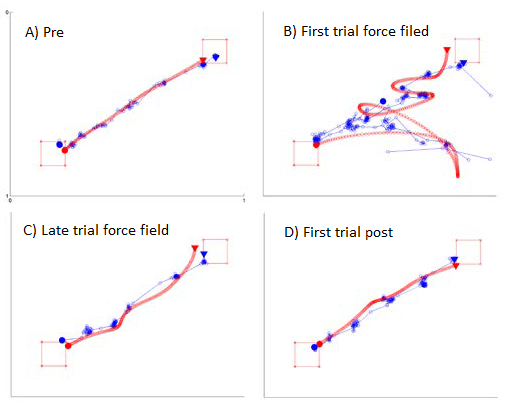
\includegraphics[width=\textwidth]{task1.png}
\caption{Task 1 path following}
\label{fig:task1}
\end{minipage}
\begin{minipage}{0.48\textwidth}
\centering
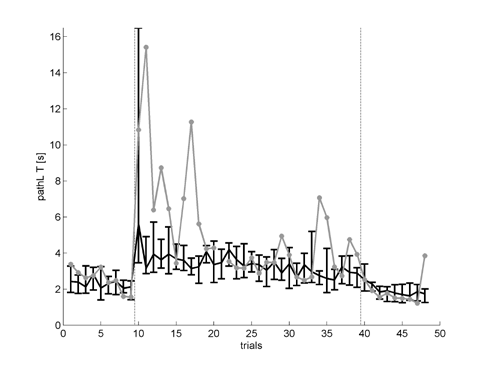
\includegraphics[width=\textwidth]{task1_pT.png}
\caption{Task 1 pathLxT vs n of trials}
\label{fig:task1_pT}
\end{minipage}
\end{figure}

During the second task there is a significant difference between \gls{td} (TD) children and children with ASD and between the first and the second attempt:
\begin{itemize}
\item Even though there is not a strong correlation among the children of a same group, it can be noticed that both TD children and ASD children performed better during the second attempt, when they already knew the path to follow a priori;
\item In general, \gls{td} children had better performance than \gls{asd} children;
\item For ASD children, the \textit{hand-gaze} distance was higher than for TD children, but quite the same in both the attempts.
\end{itemize}

Figure \ref{path} shows an example of trial with a TD child.

\begin{figure}
\centering
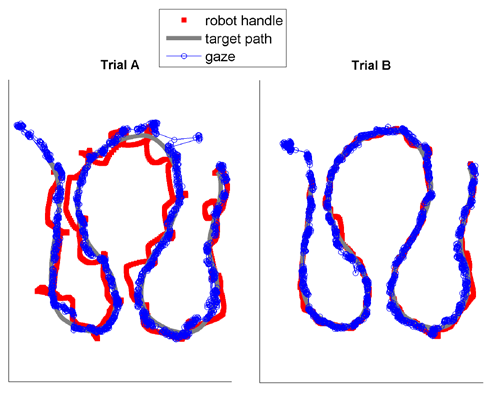
\includegraphics[width = .55\textwidth]{path.png}
\caption{Trials A and B for a \gls{td} child}
\label{path}
\end{figure}

\subsubsection{summary observations}
\label{sec:summary}

The experiment results can be summarized with a few crucial conclusions:
\begin{itemize}
\item the first task showed how children with \gls{asd} took longer to learn the task execution correctly, even though once the process had been assimilated the execution was correct, this meaning that these children showed a delayed ability to learn from sensory prediction errors; moreover the ASD child had more variability in motor execution, this suggesting more difficulty in maintaining performance consistency, and the gaze pattern was sticking less to the hand pattern if compared to the \gls{td} children.
\item the second task showed how children with ASD obtained performance slightly worse than the TD children, but anyway they were able deploy the information regarding the previously assimilated path to improve the performance. This suggests that gls{asd} children are able to take advantage of the availability of the whole motor plan and supports the hypothesis that simple motor planning is intact but there is a diminished use of feedback.
\end{itemize}

From these results, since the timing (which is strictly associated with adaptation and prediction) is one of the crucial aspects managed by the cerebellum (known to be the cerebral section reporting the most consistent brain differences in autism), it can be supported the hypothesis that bad timing in sensory integration causes degraded motor performance and delayed learning in children with \gls{asd}.

Such dysfunctions could affect not only motor processes but also cognitive ones, and this form of motor tracking could also be useful to better understand the mechanism at the basis of the well-documented visuo-motor impairments in ASD (\cite{Chow2010}, \cite{Green2013}, \cite{Papa}) and throw more light on the functional integrity of brain networks during development in people with ASD.

\section{Therapeutical techniques}
\label{sec:thera_tech}

The classical way to conduct a therapy session is a face-to-face meeting between the subject and the therapist.
Usually, it is conducted in four phases: the first one is called \textit{Instruction}, in which the therapist explains what is the skill that the subject is going to learn; the second one is the \textit{Modeling} phase, in which the therapist shows the patient what he has to do; then there is the \textit{Rehearsal} phase, in which the patient tries to imitate the therapist, and finally a \textit{Feedback} phase in which the therapist draws its own conclusions about the test.
The problem of this kind of therapy structure is the completely subjective evaluation procedure carried out by the therapist and the non-immediate subject's attention.

%TODO Avatar-based techniques to improve the performances of the therapy
%TODO Methods to detect the anxiety level
To improve the performance of the sessions, the use of \gls{va} platforms has been introducted.
A \gls{va} platform consists of an avatar, that can be a robot or a virtual character, a learning software that receives information from the Avatar, elaborates them and adjusts the response of the Avatar, and an interface for the therapist that interprets the results.
In a \gls{va} session the therapist, with the aids of the learning software, trains the Avatar to do an action that the child has to imitate. At the same time, the child tries to imitate the Avatar learning new ways to interact with the society.
Different system has been proposed, we describe here two different solutions, one more general and one more complex and efficient.

\subsection{General AVATAR idea}
\label{sec:avatar_general}

\begin{figure}[h]
\centering

\begin{minipage}{0.48\textwidth}
\centering
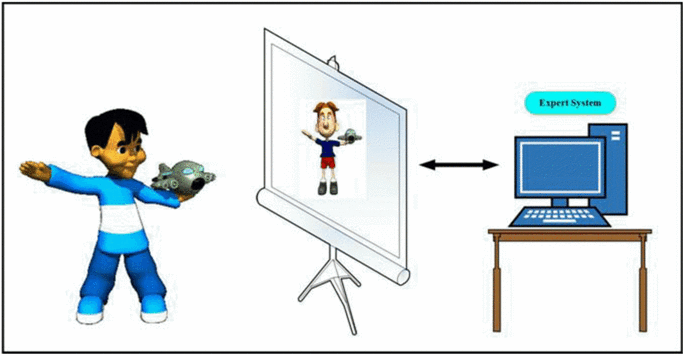
\includegraphics[width=\textwidth]{avatar_system.png}
\caption{Scheme of AVATAR system}
\label{fig:avatar_scheme}
\end{minipage}
\begin{minipage}{0.48\textwidth}
\centering
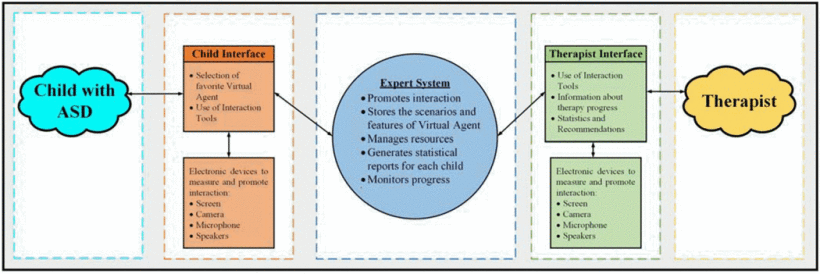
\includegraphics[width=\textwidth]{avatar_tasks.png}
\caption{Structure of AVATAR platform}
\label{fig:avatar_tasks}
\end{minipage}

\end{figure}

The idea of an Avatar-based therapy session is shown firstly in \cite{Guerrero-vasquez}. In the paper they propose a system composed by a \gls{va} and an \textit{expert system} used by the therapist to instruct the \gls{va}. A general scheme of the system is shown in \autoref{fig:avatar_scheme}.

They chose to use a Virtual Agent instead of a robot since, according with the needs, it provides the possibility to customize the tool, while a robot is limited by its structure and its \gls{dof}.

As can be seen in \autoref{fig:avatar_tasks}, the platform is organized as follows:
\begin{LaTeXdescription}
	\item[Child Interface] It selects the child's favorite Virtual Agent and uses interaction tools as screen, camera, microphone and speakers to interact with the child;
	\item[Expert System] Contains a learning algorithm that promotes interaction between the child and the Virtual Agent, it stores the scenario and features of the Virtual Agent and it monitors progress of the session in order to generate statistical reports that will be used by the therapist;
	\item[Therapist Interface] Allow the therapist to access to the reports generated by the Expert System and gives information about the current therapy, in order to allow the therapist to draw conclusions.
\end{LaTeXdescription}

The choices about the best \gls{va} to use during the sessions, or the characteristics that has to be changed in the current \gls{va}, are taken monitoring the reaction of the child when he is put in front of them.
It is not necessary for the character to be a human, since the highest degree of affinity can be towards an animal or an object.

The key point in this work is that the information received on the screen of the therapist interface shows a real time image of the child and monitored progress statistics.
Since the VA that the child observes on his screen is his therapist in disguise, actually it is the therapist who, combined with artificial intelligence, promotes the interaction in combination with the expert system.

\subsection{A more complex system}
\label{sec:avatar_complex}

Another more complex and complete approach was performed in \cite{Alahbabi17}, using a robot instead of a \gls{va}; this because it has been shown in \cite{Pioggia08} that patients manifest a more favorable response towards humanoid robots than to other non-humanoid virtual characters.

This approach has sensible advantages but also some intrinsic shortcomings:
\begin{itemize}
	\item most of the robotic or virtualized therapies are preprogrammed and this makes the session boring and repetitive;
	\item robots are limited and work in a controlled environment;
	\item usually robots do not have a quantitative behavioral analysis tool, due to the absence of therapists during their development process.
\end{itemize}

\section{Conclusions}\label{sec:conclusions}


\bibliographystyle{IEEEtran}
\bibliography{IEEEabrv,bibliography}

\end{document}
